\documentclass[xcolor=table, aspectratio=1610]{beamer}
\hypersetup{pdfpagemode=FullScreen}
\usetheme[secheader,compress]{Madrid} %Primary theme

\usepackage{verbatim}
\usepackage{graphicx}
\usepackage{tcolorbox}
\usepackage{multimedia}
\usepackage{pdfpc}
\usepackage{hyperref}
\usepackage{animate}
%% UTM Colors
\definecolor{UTMblue}{rgb}{0.043137, 0.137254, 0.254901}
\definecolor{UTMorange}{rgb}{1.0, 0.509803, 0}

\setbeamercolor{palette primary}{bg=UTMblue,fg=white}
\setbeamercolor{palette secondary}{bg=UTMblue,fg=white}
\setbeamercolor{palette tertiary}{bg=UTMblue,fg=white}
\setbeamercolor{palette quaternary}{bg=UTMblue,fg=white}
\setbeamercolor{structure}{fg=UTMblue} % itemize, enumerate, etc
\setbeamercolor{section in toc}{fg=UTMblue} % TOC sections
\setbeamercolor{title}{fg=UTMorange}
\setbeamercolor{subsection in head/foot}{bg=UTMorange,fg=white}


\setbeamertemplate{footline}
{
  \leavevmode%
  \hbox{%
    \begin{beamercolorbox}[wd=.33\paperwidth,ht=2.25ex,dp=1ex,center]{author in head/foot}%
      \usebeamerfont{author in head/foot} J.~Chamberlain \& A.~Lum
    \end{beamercolorbox}%
    \begin{beamercolorbox}[wd=.44\paperwidth,ht=2.25ex,dp=1ex,center]{title in head/foot}%
      \usebeamerfont{title in head/foot}%
      \parbox{\linewidth}{\centering Revitalizing Solar Insights: A Dashboard for WTSF}
    \end{beamercolorbox}%
    \begin{beamercolorbox}[wd=.23\paperwidth,ht=2.25ex,dp=1ex,right]{date in head/foot}%
      \usebeamerfont{date in head/foot} \insertdate \hspace*{1em} \insertframenumber{} / \inserttotalframenumber\hspace*{1ex}
    \end{beamercolorbox}%
  }%
  \vskip0pt%
}


%\setbeamertemplate{footline}
%%%%%%%%%%% BEGIN MACROS %%%%%%%%%%%%%%%%%%
% frameT: Frame with title
\newcommand{\frameT}[2]{\frame{\frametitle{#1} #2}}

% frameF: Fragile frame with title
\newcommand{\frameF}[2]{
  \begin{frame}[fragile]
    \frametitle{#1}
    #2
  \end{frame}
}

% frameTop: Frame aligned t the top
\newcommand{\frameTop}[2]{\frame[t]{\frametitle{#1} #2}}


\newcommand{\tab}{\hspace{1cm}}

\newcommand{\spaceor}{\hspace{5pt} \textbf{or} \hspace{5pt}}

%%%%%%%%%%% END MACROS %%%%%%%%%%%%%%%%%%%%
%%%%%%%%%%%%%%%%%%%%%%%%%%%%%%%%%
%
%   SLIDES BEGIN HERE           %
%
%%%%%%%%%%%%%%%%%%%%%%%%%%%%%%%%%
\begin{document}

\title{Revitalizing Solar Insights: \\ A Dashboard for West Tennessee Solar Farm}

\author{Joshua Chamberlain \& Andy Lum \\ \vspace{0.1in} Mentor: Dr.~Justin R.~Sims}
\institute{UT Martin}
\date{\today}

%%%%%%%%%%%%%%%%%%%%%%%%%%%%%%%%%
%
%    BACKGROUND                 %
%
%%%%%%%%%%%%%%%%%%%%%%%%%%%%%%%%%
\frame{\titlepage}
\frameT{Background}{    
    \Large \textbf{The West Tennessee Solar Farm}
    \begin{itemize}
        \item<1-> \Large Located in Stanton, TN: 1 hour Northwest of Memphis
        \item<2-> \Large Generates 5-megawatts of power with over 25 acres of solar panels.
        \only<3->{
            \begin{center}
                \includegraphics[width=0.7\linewidth, height=0.6\textheight]{WTSF.pdf}
            \end{center}
        }
    \end{itemize}
}
%%%%%%%%%%%%%%%%%%%%%%%%%%%%%%%%%
%
%   TABLE OF CONTENTS           % ----- OMITTED FOR NOW
%
%%%%%%%%%%%%%%%%%%%%%%%%%%%%%%%%%
% \frametitle{Table of Contents} 
% \begin{enumerate}
%     \item Introduction
%     \begin{itemize}
%         \item Motivation
%     \end{itemize}

%     \item R-Shiny \& Functionalities

%     \item List of Technologies
%     \begin{itemize}
%         \item Technologies used to supply the dashboard
%     \end{itemize}

%     \item Project Goals
%     \begin{itemize}
%         \item What do we want to accomplish overall?
%     \end{itemize}

%     \item Dashboard Demo

%     %\item Results
%     %\begin{itemize}
%         %\item What went well? What didn't go well?
%     %\end{itemize}

%     \item Conclusion
%     \begin{itemize}
%         \item Future Work
%         \item What did we accomplish? What did we learn?
%     \end{itemize}

% \end{enumerate}
% \end{frame}

%%%%%%%%%%%%%%%%%%%%%%%%%%%%%%%%%
%
%   INTRODUCTION / MOTIVATION   %
%
%%%%%%%%%%%%%%%%%%%%%%%%%%%%%%%%%
\frameT{Introduction}{
    \vfill 
    \begin{block}{Motivation}
     \Large Can we build an interactive dashboard to:
     \bigskip
     \begin{enumerate}
         \item \Large Improve research and education accessibility
         \bigskip
         \item \Large Optimize power production
         \bigskip
         \item \Large Advance sustainable energy practices
         \bigskip
     \end{enumerate}
    \end{block}
    \vfill
}
%%%%%%%%%%%%%%%%%%%%%%%%%%%%%%%%%
%
%   R-SHINY & FUNCTIONALITIES   %
%
%%%%%%%%%%%%%%%%%%%%%%%%%%%%%%%%%
\section{}
\frameT{R-Shiny \& Functionalities}{
    \begin{enumerate}
        \item<1-> \Large Provides an easier and more integrated way to creating web-based dashboards, allowing us to concentrate on design aspects, while abstracting the complexities of web development languages.
        \bigskip
        \item<2-> \Large Provides the following functionalities:
        \begin{itemize}
            \item<3-> \Large Real-Time Data Visualization
            \begin{itemize}
                \item <3-> \Large Interactive Maps
                \item <3-> \Large Sensor Information Panel
                \item <3-> \Large Historical Data Analysis
                \item <3-> \Large Exporting Data
            \end{itemize}
            \bigskip
            %\item<4-> Interactive Maps
            %\item<5-> Sensor Information Panel
            %\item<6-> Historical Data Analysis
            \item<4-> \Large User-Friendly Interface
            %\item<8-> Responsive Design
            %\item<9-> Dashboard Hosting
            %\item<10-> Exporting Data
        \end{itemize}
    \end{enumerate}
}
%%%%%%%%%%%%%%%%%%%%%%%%%%%%%%%%%
%
%   TECHNOLOGIES                %
%
%%%%%%%%%%%%%%%%%%%%%%%%%%%%%%%%%
\section{}
\frameT{Technologies}{
  \begin{enumerate}
      \item<1-> \large\textbf{MySQL}\par
      Stores and manages sensor data in a table containing minute by minute data separated by data for each sensor.
      \item<2-> \large\textbf{Python}\par
      Retrieves data from the MySQL database and updates a Google Drive CSV for data simulation.
      \item<3-> \large\textbf{R-Shiny}\par
      Develops an interactive dashboard for data visualization.
      \item<4-> \large\textbf{Shinyapps.io}\par
      Hosts a web server to allow users from all major operating systems to be able to access the dashboard.
      \item<5-> \large\textbf{Google Cloud Console}\par
      Safeguards API information for enhanced data security.
  \end{enumerate}
}
%%%%%%%%%%%%%%%%%%%%%%%%%%%%%%%%%
%
%   PROJECT GOALS               %
%
%%%%%%%%%%%%%%%%%%%%%%%%%%%%%%%%%
\section{}
\frameT{Project Goals} {
  \begin{enumerate}
      \item<1-> \Large\textbf{Streamlined Data Pipeline}
      %Achieve efficiency by establishing a robust data pipeline from MySQL to Python, culminating in organized data storage within Google Drive's CSV format, seamlessly facilitating further analysis within the R-Shiny environment.
      \item<2-> \Large\textbf{Continuous Data Maintenance}
      %Elevate data integrity through the implementation of an automated Python script, equipped with comprehensive error handling capabilities, ensuring the continuous and real-time updating of Google Drive's CSV repository to provide a reactive data environment.
      \item<3-> \Large\textbf{R-Shiny Dashboard}\par
      Encompasses all of the aforementioned functionalities.
      \item<4-> \Large\textbf{Cross-Platform Accessibility}\par 
      Ensure inclusivity by designing a webpage that accommodates diverse laptop operating systems, guaranteeing a seamless user experience.

        \bigskip
  \end{enumerate}
}
%%%%%%%%%%%%%%%%%%%%%%%%%%%%%%%%%
%
%   INITIAL MOCKUP              %
%
%%%%%%%%%%%%%%%%%%%%%%%%%%%%%%%%%
\frameT{Initial Mockup}{
\vspace{-1cm}
\centering
\includegraphics[scale = 0.45]{Initial Mockup.pdf}
}
%%%%%%%%%%%%%%%%%%%%%%%%%%%%%%%%%
%
%   DASHBOARD DEMO              %
%
%%%%%%%%%%%%%%%%%%%%%%%%%%%%%%%%%
\frameT{Dashboard Demo} {
   
  %\href{https://seniordesign.shinyapps.io/shiny_dashboard/}{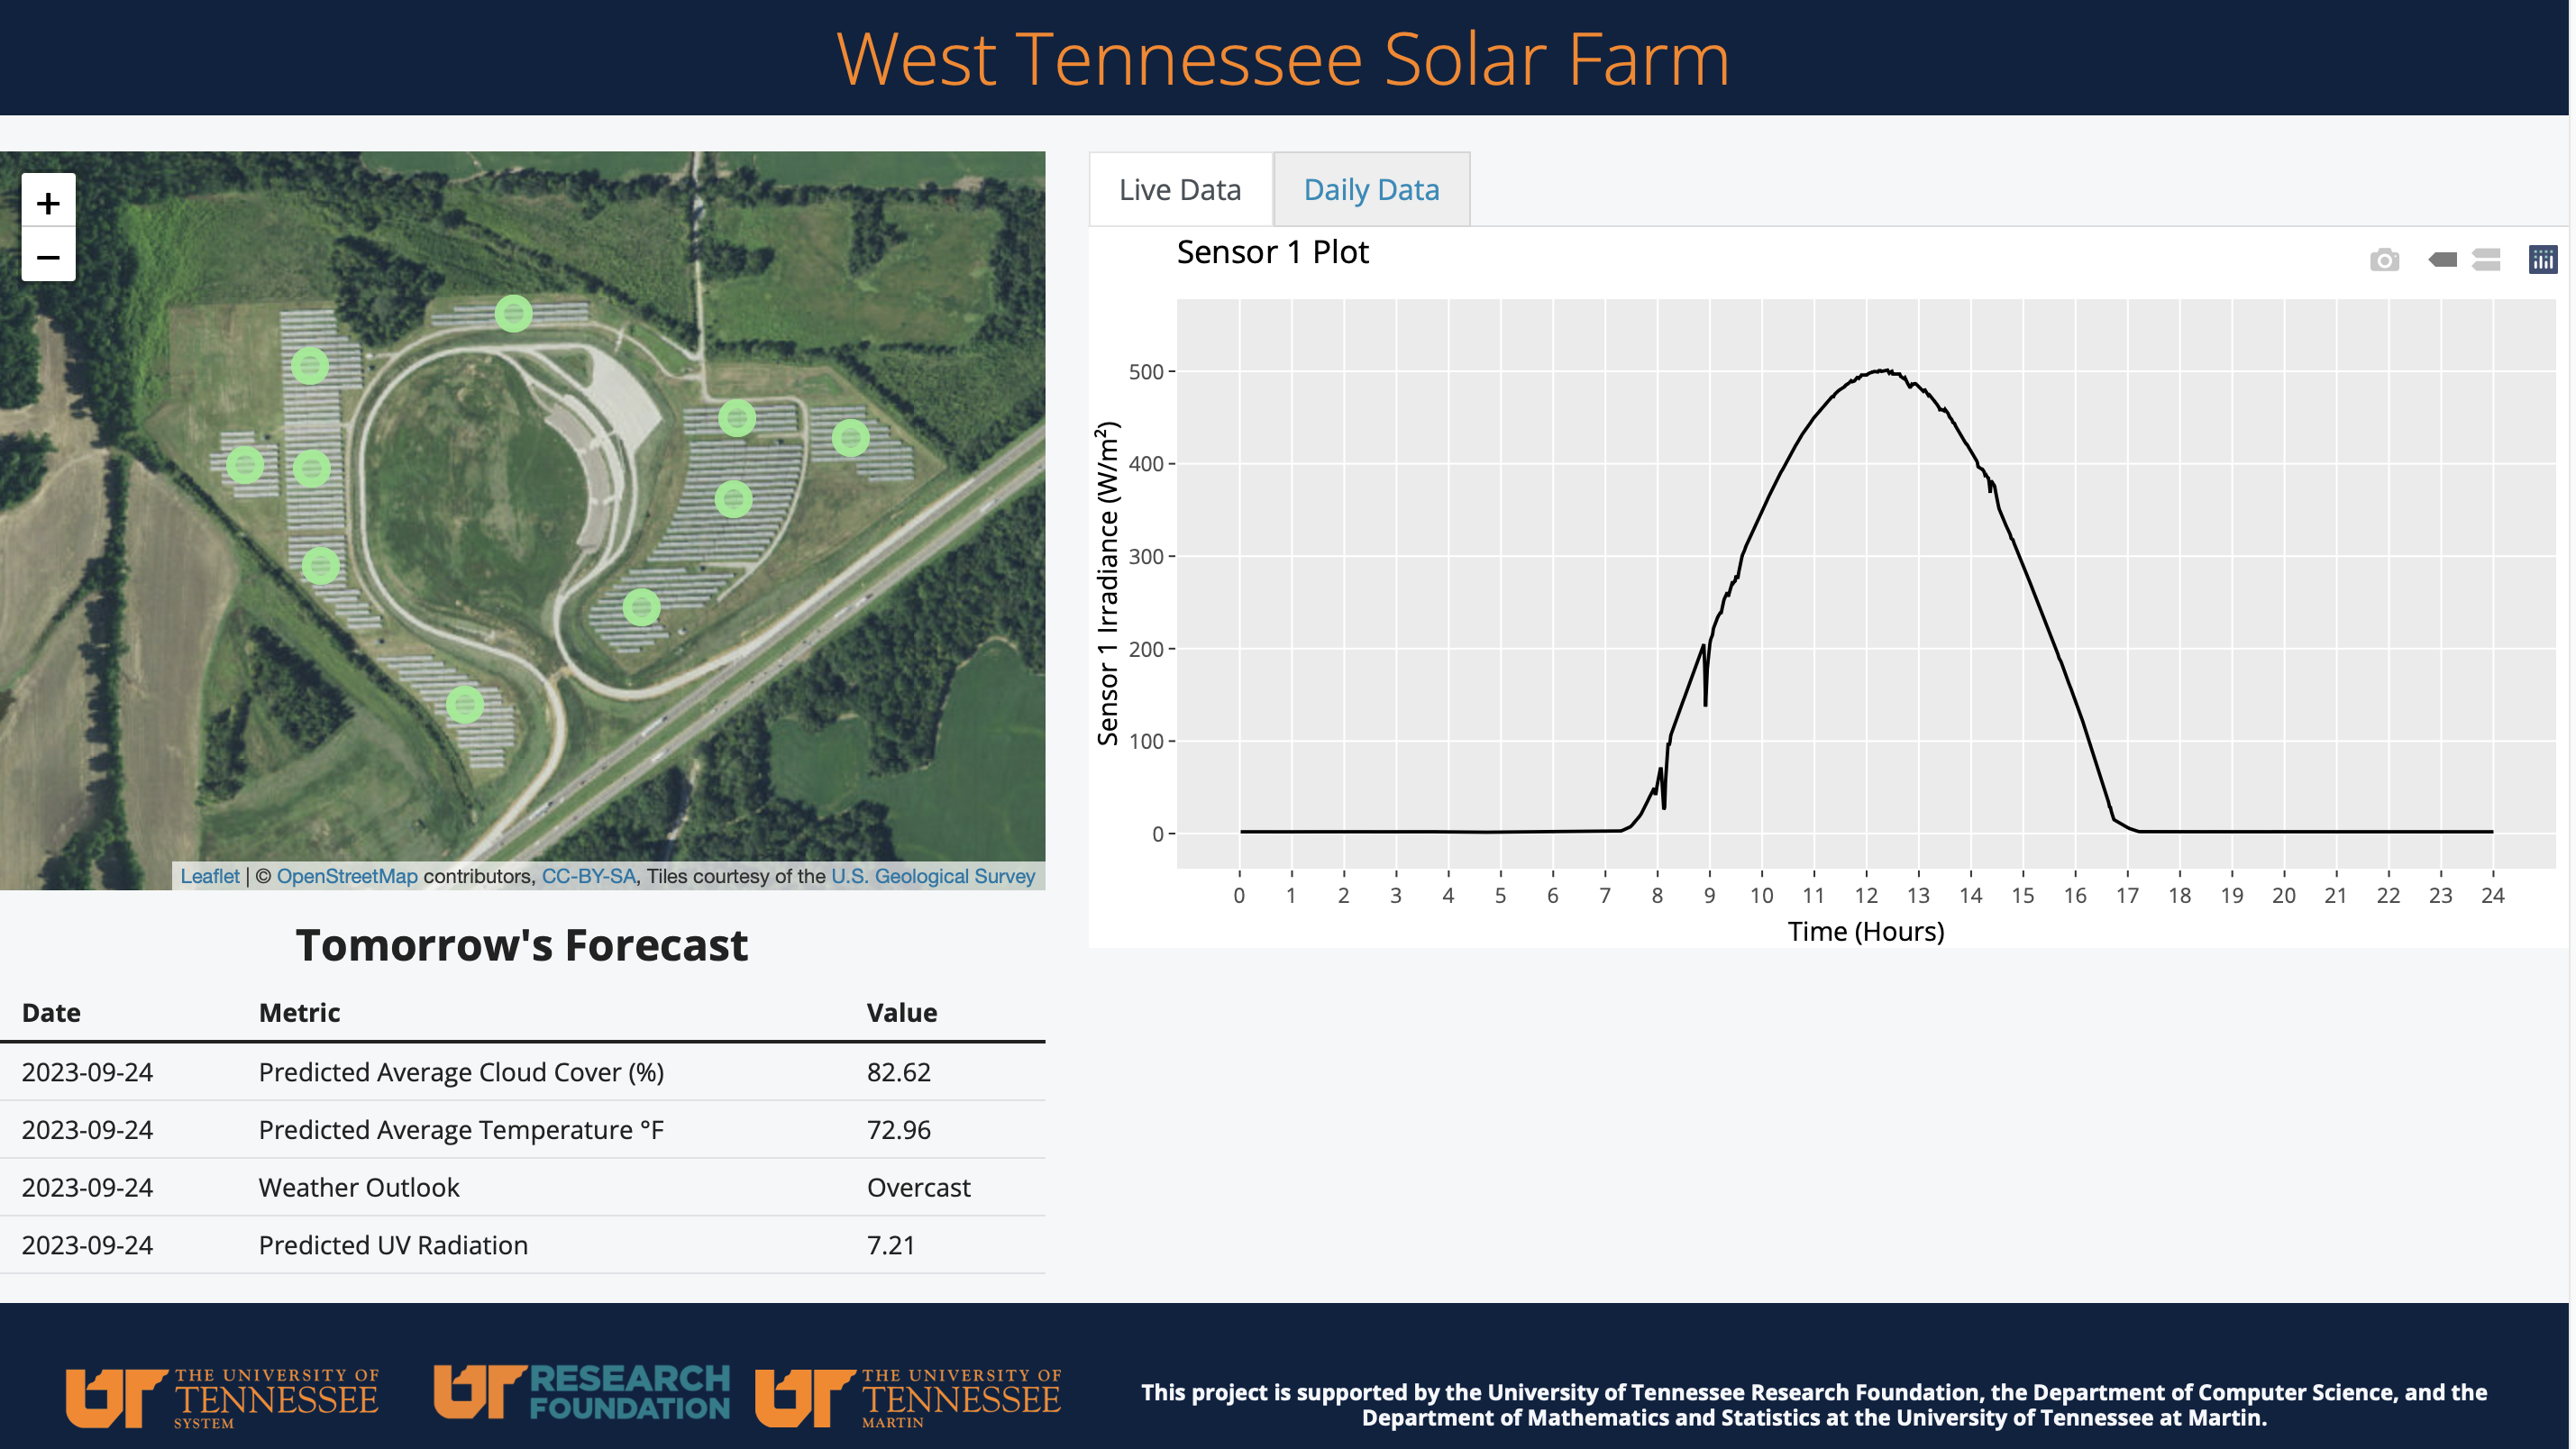
\includegraphics[width=\linewidth]{Dashboard.png}}
  %\href{https://youtu.be/hkWfeRpQ3V0}{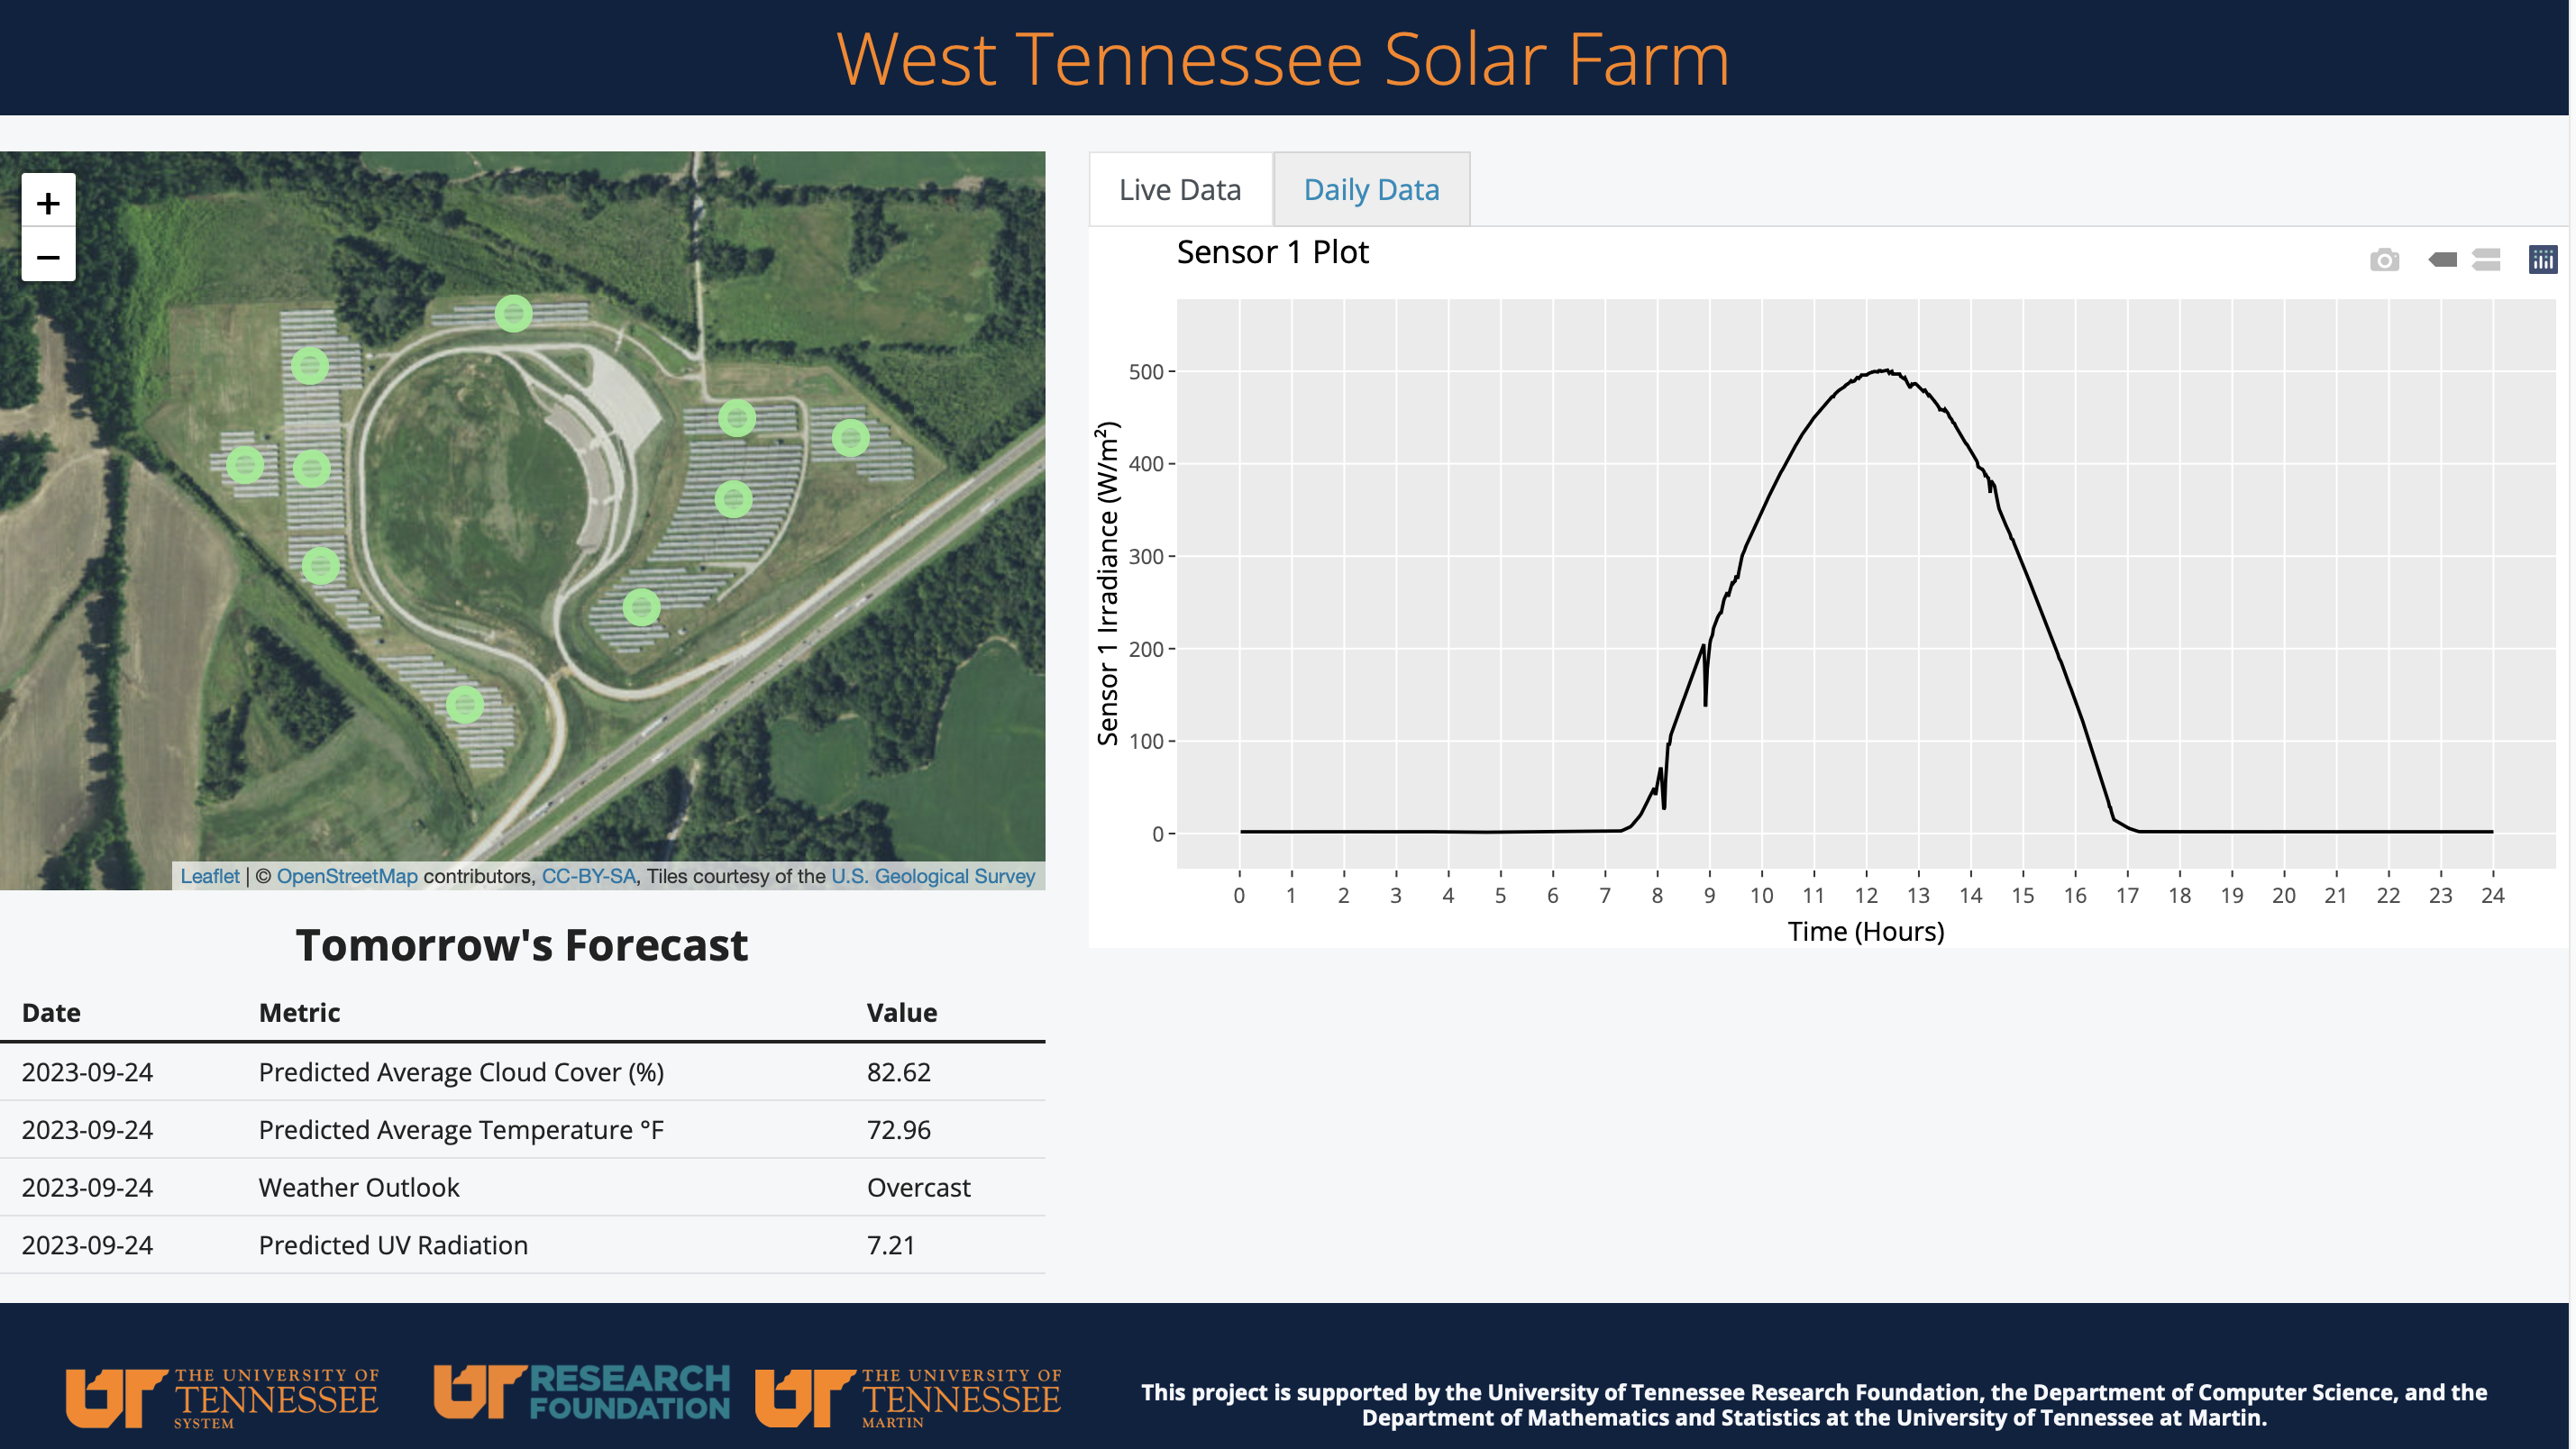
\includegraphics[width=\linewidth]{Dashboard.png}}
  %\includegraphics[width=340, height = 200]{Thumbnail.png}
  \href{https://youtu.be/EFrpsb2XRkM}{\includegraphics[width=\linewidth]{Thumbnail.png}}
}
%%%%%%%%%%%%%%%%%%%%%%%%%%%%%%%%%
%
%   CHALLENGES                  %
%
%%%%%%%%%%%%%%%%%%%%%%%%%%%%%%%%%
\frameT{Challenges} {
    \begin{enumerate}
        \item<1-> \Large\textbf{Establishing a streamlined data flow}
        \begin{itemize}
            \item<1-> \Large mySQL $\Rightarrow$ Python $\Rightarrow$ Google Drive $\Rightarrow$ R-Shiny Dashboard
        \end{itemize}
        \bigskip
        \item<2-> \Large\textbf{Error-Handling}
        \bigskip
        \bigskip
        \item<3-> \Large\textbf{Webpage Development}
        \begin{itemize}
            \item<3-> \Large Accessibility across a variety of major operating systems
        \end{itemize}
        \bigskip
    \end{enumerate}
}
%%%%%%%%%%%%%%%%%%%%%%%%%%%%%%%%%
%
%   FUTURE WORK                 %
%
%%%%%%%%%%%%%%%%%%%%%%%%%%%%%%%%%
\frameT{Future Work} {
    \begin{enumerate}
        \item<1-> \Large\textbf{Predictive Analysis}
        \begin{itemize}
            \item<1-> \Large Predicting the amount of power to be produced
        \end{itemize}
        \bigskip
        \item<2-> \Large\textbf{Notifications}
        \begin{itemize}
            \item<2-> \Large Real-time alerts
        \end{itemize}
        \bigskip
        \item<3-> \Large\textbf{Video Tutorial}
        \begin{itemize}
            \item<3-> \Large Outline how to use the dashboards functionalities
        \end{itemize}
        \bigskip
    \end{enumerate}
}
%%%%%%%%%%%%%%%%%%%%%%%%%%%%%%%%%
%
%   CONCLUSION                  %
%
%%%%%%%%%%%%%%%%%%%%%%%%%%%%%%%%%
\frameT{Conclusion} {
    \Large \textbf{The dashboard provides:}\\
    \begin{enumerate}
        \Large\item An educational resource for individuals interested in learning about the solar farm process.
        \Large\item A tool that offers researchers access to public data for their research.
    \end{enumerate}
}
% \section{Results}
% \frameT{Results} {
%   Describe any results of your work here.

%   \bigskip

%   Things that worked?

%   \bigskip

%   Things that didn't work?
% }
%%%%%%%%%%%%%%%%%%%%%%%%%%%%%%%%%
%
%   CONTACT INFO                %
%
%%%%%%%%%%%%%%%%%%%%%%%%%%%%%%%%%
\section{Contact Information}
\frameT{Any Questions?} {
  

\begin{center}
  \Large Comments?
\end{center}

\bigskip

\Large More information about our Dashboard for West Tennessee Solar Farm:\\
\begin{center}
  \href{https://github.com/andylum/495-senior-design.git}{https://github.com/andylum/495-senior-design.git}
\end{center}

\bigskip

\Large
\textbf{Joshua Chamberlain}: \href{mailto:jospcham@ut.utm.edu}{jospcham@ut.utm.edu}
\bigskip

\textbf{Andy Lum}: \href{mailto:andlum@ut.utm.edu}{andlum@ut.utm.edu}

}
\end{document}
